% previous variable selection details file

\section{Normal Distributions Transformed to the Unit Simplex: The ALoVaS method. }\label{sec:ALN_chapter}

This chapter outlines the additive logistic transformation, which transforms a $d$ dimensional multivariate normal distribution onto the unit simplex in $d+1$ dimensions. Note that the unit simplex in $d+1$ dimensions actually lies in a subspace of $d$ dimensions because of the constraint that the sum of the probabilities equals one. 

The goal of this chapter is to find a transform that moves the space $\mathbb{R}^d$ \newnot{symbol:real} to the simplex $\mathbb{S}^d$. \newnot{symbol:simp} The simplex $\mathbb{S}^d$ is a space defined by the constraints $\{x_i: 0<x_i<1, \sum_{j=1}^dx_j <1 \}$, and the extra term $x_{d+1}=1-\sum_{j=1}^d x_j$ ensures the total sums to 1.  

Define the notation $\yvec$, for the normal random variables that reside in the $\Rsp{d}$  dimensional space. Define the notation $\xvec$  for the vector that resides on $\simp{d}$, the simplex in $d$ dimensions. We use an underline to indicate that the stated quantity is a column vector and capital greek letters (and $I$) will denote matrices (the identity matrix) 

\begin{equation}\label{eqn:simplex_transform}
x_i = \frac{e^{y_i}}{1+\displaystyle{\sum_{j=1}^de^{y_j}}}. \\
\end{equation}
The Jacobian of the transform is defined as
\newnot{symbol:jacobian}
\begin{equation}\label{eqn:jacobian}
J(\yvec \vert \xvec) = \left( \prod_{j=1}^{d+1}x_j \right)^{-1}.
\end{equation}

It is important to note that $\yvec\in\Rsp{d}$, whereas $\xvec\in\simp{d}$. The $d$ dimensional normal has the usual parameters and density

\begin{equation}\label{eqn:multinormal}
f_{\yvec}(\yvec\vert \Sigma, \mu)=(2\pi)^{-d/2}|\Sigma|^{-1/2}\exp{\left(-1/2(\yvec-\muvec)^T\Sigma^{-1}(\yvec-\muvec)\right)}.
\end{equation}

Upon applying the transformation defined by Equation \ref{eqn:simplex_transform}, we arrive at the additive logistic normal (ALN) distribution, with density 

\begin{equation}
f_{\xvec}(\xvec\vert \Sigma, \mu)=\frac{(2\pi)^{-d/2}}{\sqrt{\vert\Sigma\vert}\prod_{j=1}^{d+1}x_j } 
\exp{\left(-1/2(\text{log}(\xvec_{(d+1)}/x_{d+1})-\muvec)^T\Sigma^{-1}(\text{log}(\xvec_{(d+1)}/x_{d+1})-\muvec)\right)}.
\end{equation}
The vector notation $\xvec_{(d+1)}$ denotes the vector in $d$ dimensions that has the $d+1$ entry removed from the vector $\xvec$. 
It is important to note that this density function is defined on the space $\simp{d}$ and \emph{not} on the space $\Rsp{d}$. 

A useful property of this transform is that we can handle probabilities defined on the $d$ dimensional simplex while working with a normal distribution. This is a common and comfortable probability distribution for most statisticians and applied scientists.
We now wish to understand how the specification of the mean vector $\muvec$ and the covariance matrix $\Sigma$ impact the structure of the ALN density. From simulation we can formulate the following conclusions: 

\begin{itemize}
\item With $\Sigma=I$, increasing the mean vector in the positive direction in any one of the $d$ components individually corresponds to shifting density towards the corner of the simplex associated with that covariate. 
\item With $\Sigma=I$, increasing the mean vector in the negative in \emph{all} $d$ components corresponds to shifting density towards the $d+1$ corner of the simplex. 
\item Keeping $\muvec =\vec{0}$, adjusting any of the variances corresponds to shifting towards a projected space of $\simp{d}$. 
\item With $\muvec =\vec{0}$, making one variance small corresponds to the shifting density towards the median of the simplex associated with the remaining $d$ dimensions. 
\item Making the $\Sigma$ matrix approximately singular and moving $\muvec$ in the negative direction for all components places most of the probability density along the median of simplex associated with first $d$ dimensions. 
\item If $\Sigma = \text{Diag}(\sigma^2_j)$,\newnot{symbol:diag} as the $\sigma^2_j$ entries become smaller, the probabilities approach the CGM specification.    
\end{itemize}

Using the transformation defined in Equation \ref{eqn:simplex_transform} and the fact that it is relatively simple to simulate from the vector normal distribution, the ALN density can be simulated. 

\begin{figure}[ht]
\begin{minipage}[b]{0.45\linewidth}
\centering
\includegraphics[width=\textwidth]{mu0_0.pdf}
\caption[ALN plot with a zero mean vector]{In this figure, $\muvec$ has all zero entries, with $\Sigma=I$, corresponding to the equiprobable case. Each probability is approximately $1/(d+1)$. }
\label{fig:figure9}
\end{minipage}
\hspace{0.5cm}
\begin{minipage}[b]{0.45\linewidth}
\centering
\includegraphics[width=\textwidth]{mu-1-1.pdf}
\caption[ALN plot with a negative one mean vector]{In this figure, $\vec{\mu}=(-1,-1)^T$, with $\Sigma=I$, corresponds to moving towards a sparser set of covariates. }
\label{fig:figure10}
\end{minipage}
\end{figure}

\begin{figure}[ht]
\begin{minipage}[b]{0.45\linewidth}
\centering
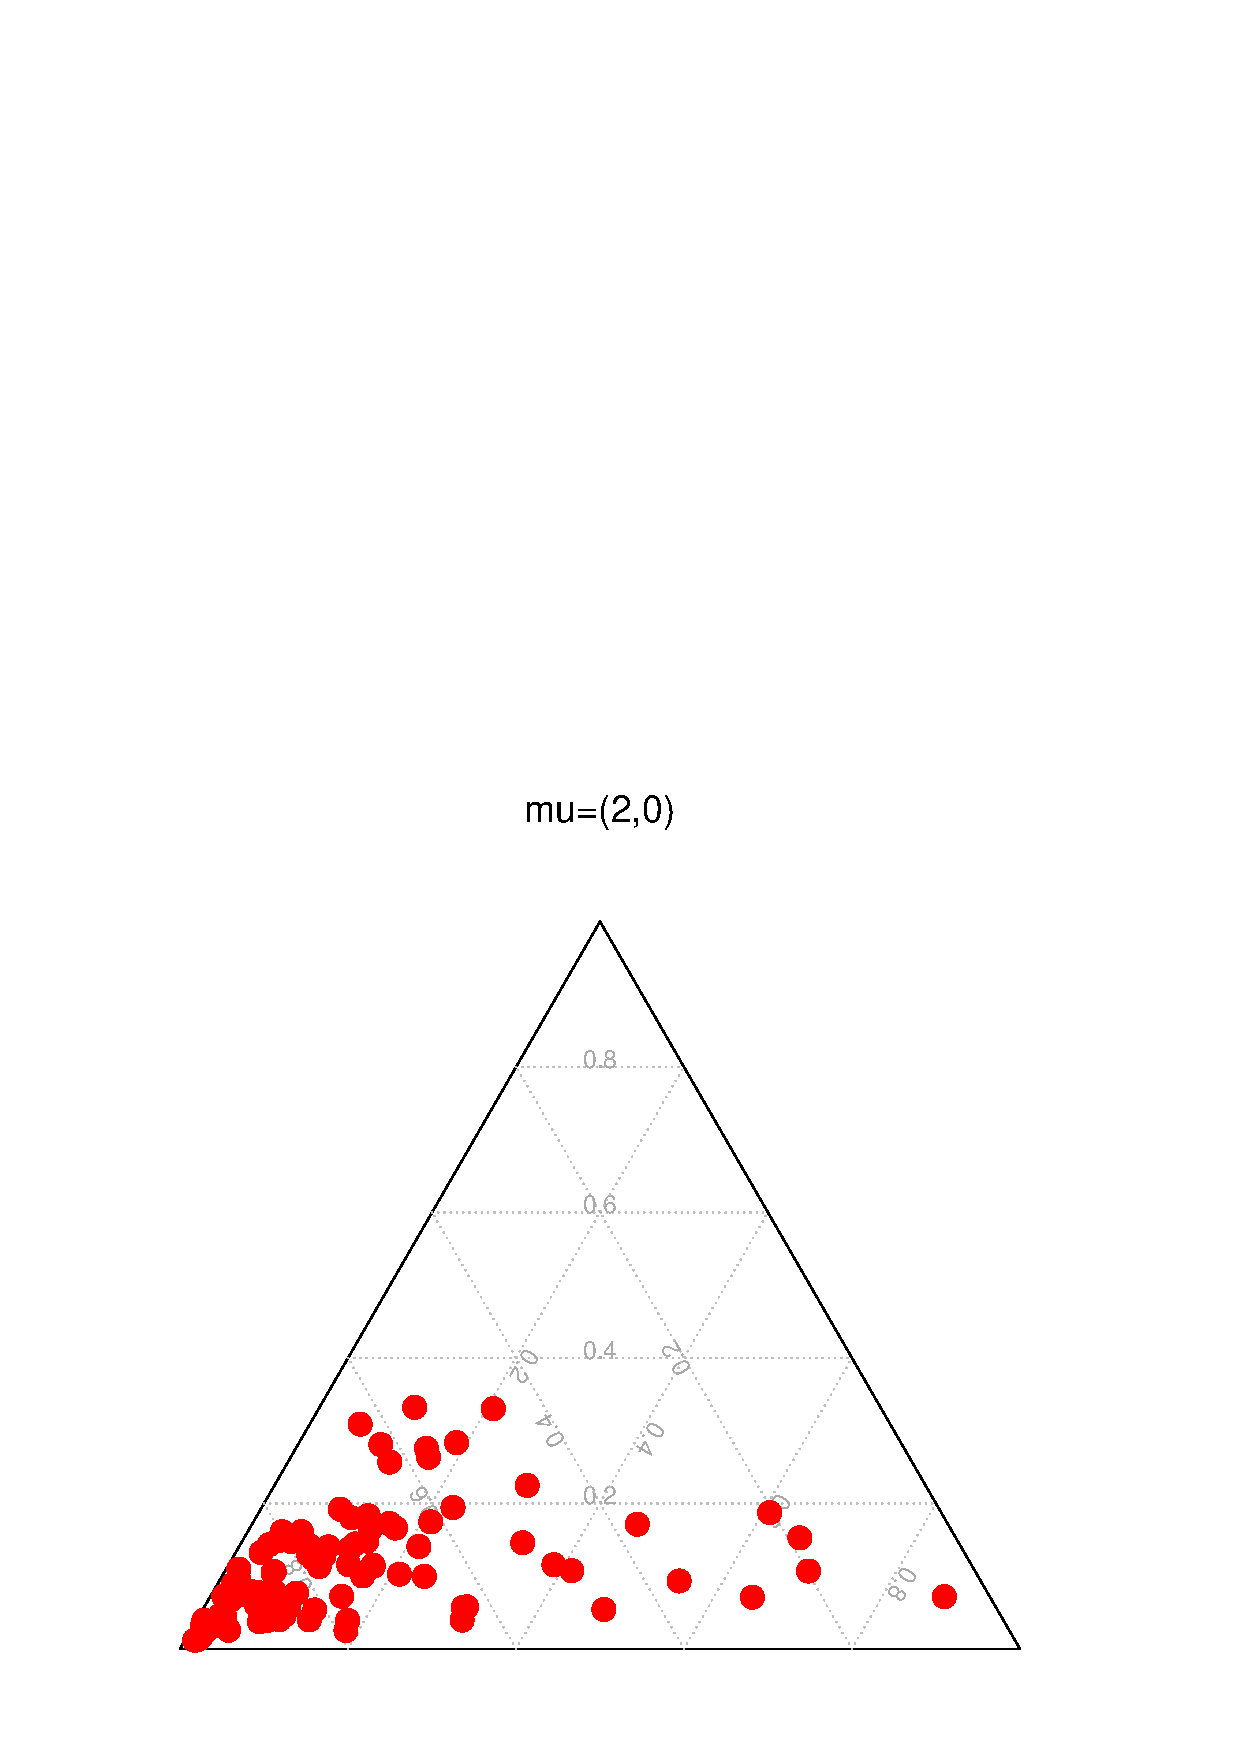
\includegraphics[width=\textwidth]{mu2_0.pdf}
\caption[ALN plot with a mean vector $(2,0)^{T}$]{$\vec{\mu}=(2,0)^T$, with $\Sigma=I$, moves the density towards one corner of the simplex. }
\label{fig:figure1}
\end{minipage}
\hspace{0.5cm}
\begin{minipage}[b]{0.45\linewidth}
\centering
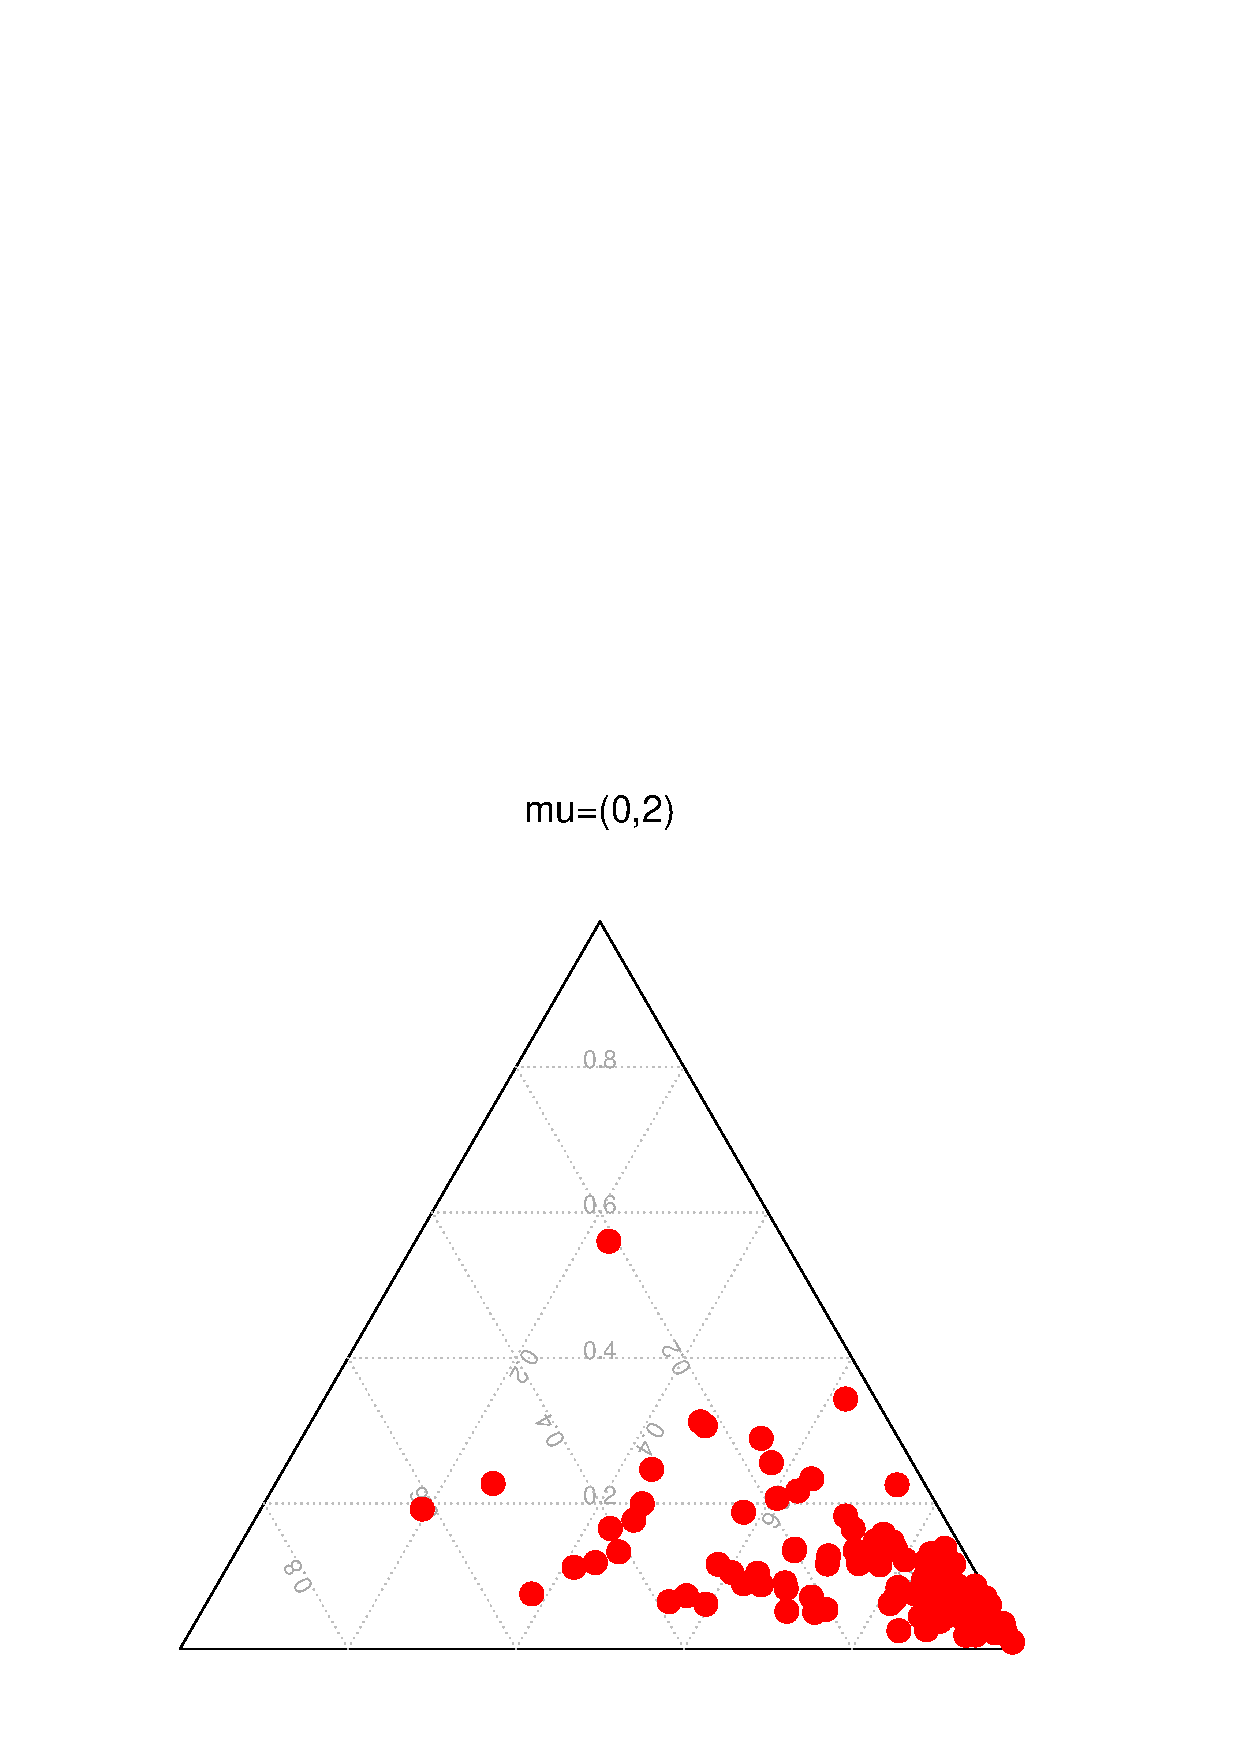
\includegraphics[width=\textwidth]{mu0_2.pdf}
\caption[ALN plot with mean vector $(2,0)^{T}$]{$\vec{\mu}=(0,2)^T$, with $\Sigma=I$, moves the density towards the other corner of the simplex. }
\label{fig:figur2}
\end{minipage}
\end{figure}

\begin{figure}[ht]
\begin{minipage}[b]{0.45\linewidth}
\centering
\includegraphics[width=\textwidth]{mu-2_2.pdf}
\caption[ALN plot with a mean vector of $(-2,2)^{T}$]{$\vec{\mu}=(-2,2)^T$, with $\Sigma=I$, corresponds to most probability mass along a corner of the simplex and is a sparse representation.} 
\label{fig:figure3}
\end{minipage}
\hspace{0.5cm}
\begin{minipage}[b]{0.45\linewidth}
\centering
\includegraphics[width=\textwidth]{Sigma0_01_10.pdf}
\caption[ALN plot $\Sigma=\text{Diag(0.01,100)}$]{ $\vec{\mu}=\vec{0}$, with
 $\Sigma= \text{diag}(0.01, 100)$, corresponds to most density lying on a one dimensional subspace (the second covariate in the $\Rsp\ $ space).  }
\label{fig:figure4}
\end{minipage}
\end{figure}


\begin{figure}[ht]
\begin{minipage}[b]{0.45\linewidth}
\centering
\includegraphics[width=\textwidth]{Sigma1_9_9_1.pdf}
\caption[ALN plot $\Sigma$ numerically singular]{Here $\Sigma$ is approximately singular and most of the probability mass in concentrated along the $d+1$th dimension in the $\mathbb{R}^{d+1}$ space.  }
\label{fig:figure5}
\end{minipage}
\hspace{0.5cm}
\begin{minipage}[b]{0.45\linewidth}
\centering
\includegraphics[width=\textwidth]{Sigma10_0_01.pdf}
\caption[Similar to the case in Figure \ref{fig:figure4} but with the variances reversed]{Similar to the case in Figure \ref{fig:figure4} but with the variances reversed.}
\label{fig:figure6}
\end{minipage}
\end{figure}

 \begin{figure}[ht]
\begin{minipage}[b]{0.45\linewidth}
\centering
\includegraphics[width=\textwidth]{Sigma100_100.pdf}
\caption[ALN plot with a zero vector mean and $\Sigma=\text{Diag}(100,100)$]{$\vec{\mu}=\vec{0}$, with
 $\Sigma= \text{diag}(100, 100)$, corresponds to encouraging sparse representations \emph{a priori}.  }
\label{fig:figure7}
\end{minipage}
\hspace{0.5cm}
\begin{minipage}[b]{0.45\linewidth}
\centering
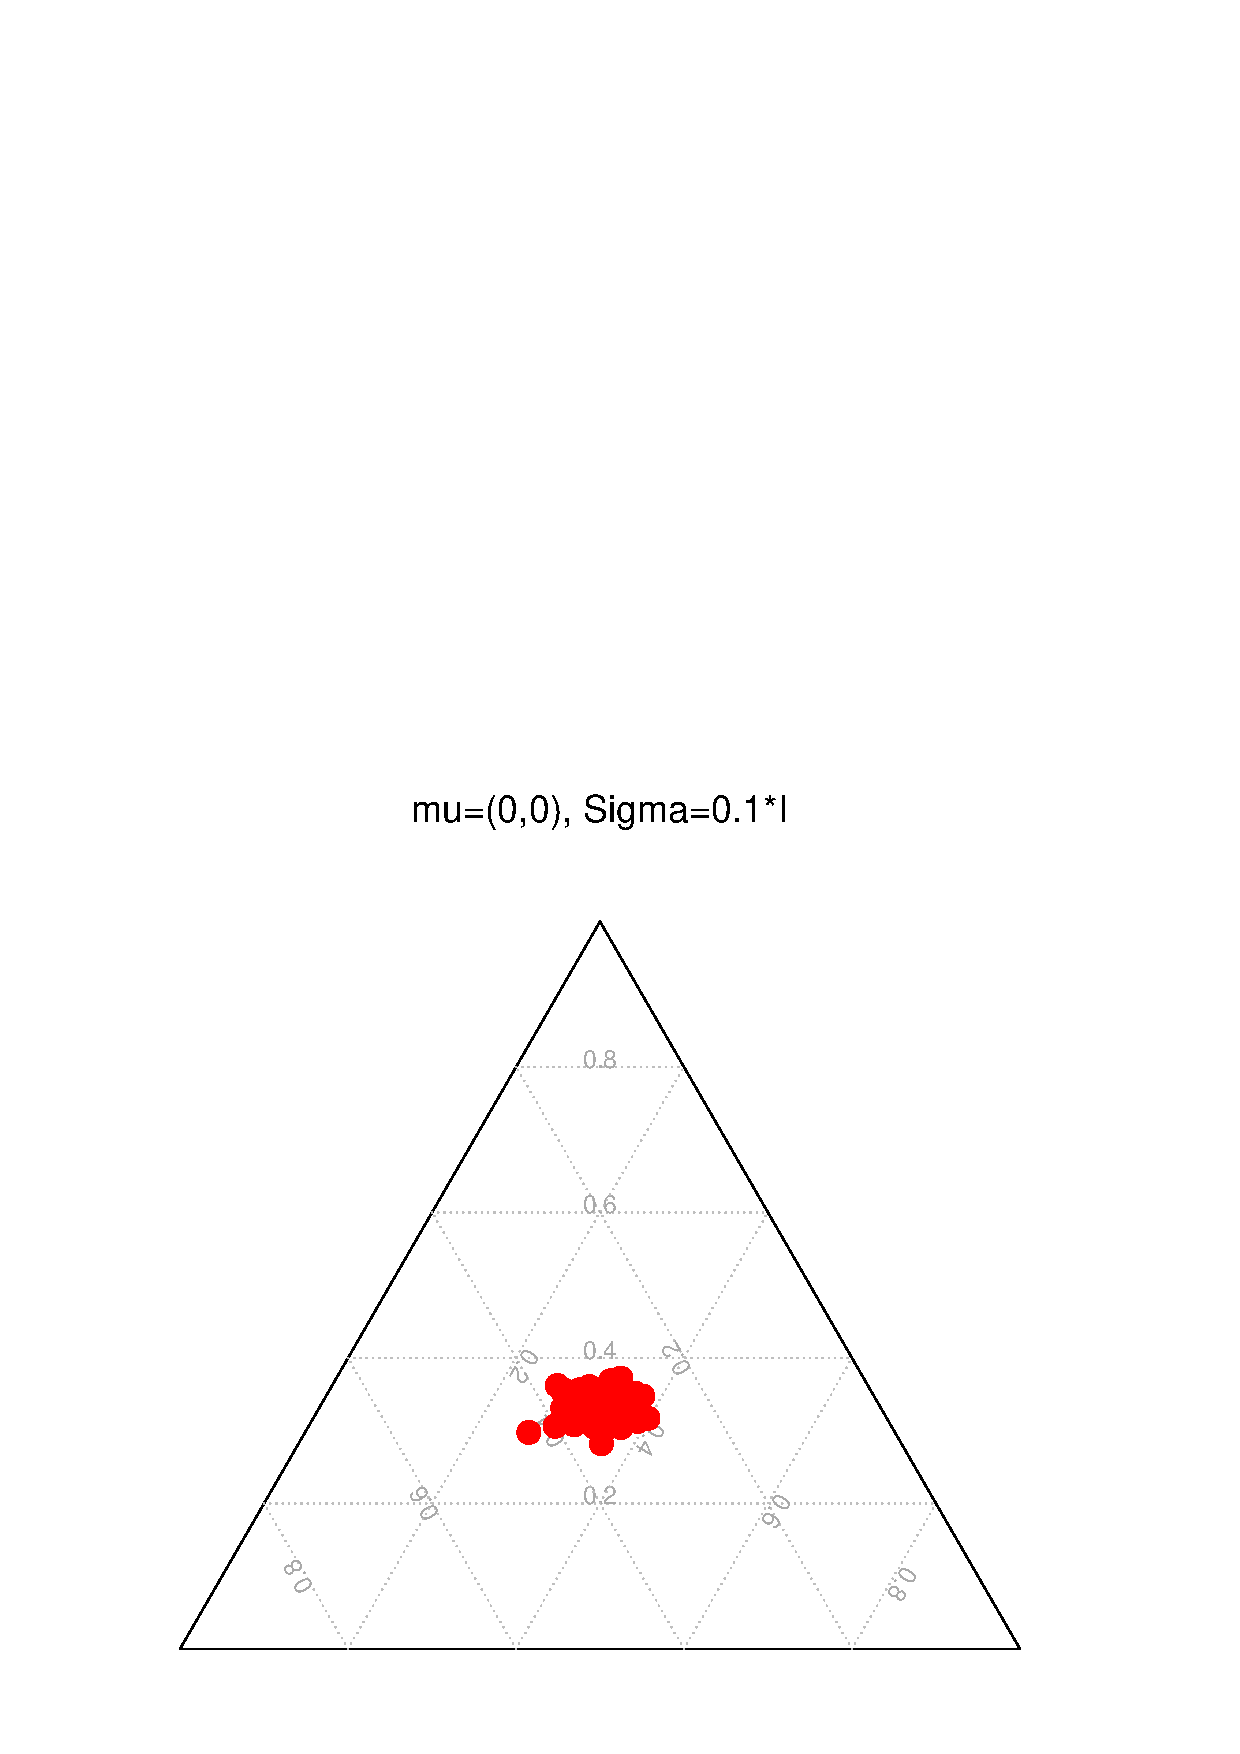
\includegraphics[width=\textwidth]{Sigma01_01.pdf}
\caption[ALN plot approximating the CGM model]{Here $\Sigma=0.1I$, and $\muvec=\vec{0}$, corresponds to roughly the CGM specification.}
\label{fig:figure8}
\end{minipage}
\end{figure}

 The simulations indicate that we can scale everything at approximately an $\mathcal{O}(d)$\newnot{symbol:big_oh} rate because of the diagonality of the variance covariance matrix, no matrix inversions are required. The step that remains is to link this portion of the model with the (currently) observed data in the tree, so that better trees are favored over trees that are worse, when each is observed in the Markov chain. We will first work in the space $\Rsp{d}$ and then translate to probabilities by using Equation \ref{eqn:simplex_transform}.  
 
 If we are to focus on the means and a collection of variances in a multivariate normal i.i.d. model, then we must fully specify the likelihood and the prior to form our posterior. 
 
 The likelihood of the tree is defined as follows: the tree's selected covariates are counted and summed across all observed splits, leading to a likelihood taking on discrete values for the observed data. Let us define a multiplier that can take on an arbitrary positive or negative value in a compact region. We then multiply the counts of splits on each covariate by this quantity, effectively creating a mean which can take on arbitrary values in $\Rsp{}$. 

\subsection{A Simple Sampler Approach}

This subsection derives the full conditional densities for each necessary update in the Gibbs loop to sample posterior weights on each dimension in the CGM decision tree sampler. 
 Throughout this subsection we will use the notation $\odot$\newnot{symbol:hadamard} to denote a Hadamard product of two matrices or vectors. 
 
 \subsubsection{The General Strategy}
 There are many problems with using a Dirichlet prior and a Multinomial conjugate likelihood. The two most glaring problems are the implicit prior assumption of same scales on each covariate and the fact that all covariances or, equivalently, correlations must be negative. If the generative model of the data is a linear model with an interaction term and a decision tree model is fit to the data, then several splits will occur on the two interacting covariates. These splits will occur alternately until the curvature is sufficiently approximated \cite{ishwaran2010high}. This situation indicates a positive correlation between the two covariates. Higher order interactions will result in similar positive correlations between collections of covariates. Therefore we conclude the Dirichlet density as a posterior for the probability of selecting a covariate is an inferior model. Moreover, the initial motivation for modeling data with a decision tree was to handle survey data that contained many complex interactions that would be too computationally expensive to evaluate using linear model methods \cite{morgan1963problems}. 
 
 The likelihood will be denoted by
 
 \begin{equation}\newnot{symbol:mvn}
 MVN(\vec{c}\odot\vec{s}\vert \vec{\mu}, \Sigma=\text{Diag}(\sigma^2_j)).
 \end{equation}
 
 The prior is also a normal 
 
 \begin{equation}
 \pi(\vec{\mu}\vert \vec{\mu}_p, \Sigma)=MVN(\vec{\mu}\vert \vec{\mu}_p, \Sigma).
 \end{equation}

The priors on the variances are \iid $\sim \invgam{\sigma_j^2}{a_j}{b_j}$.
Finally the priors on the $c_j$s are \iid\ scaled beta's with densities 

\begin{equation}\newnot{symbol:scaled_beta}
S\beta(c_j\vert \alpha_j, \beta_j, -a, a)\equiv\pi(c_j\vert \alpha_j, \beta_j, -a, a)= \frac{(c_j+a)^{\alpha_j-1}(a-c_j)^{\beta_j-1}\Gamma(\alpha_j+\beta_j)}{(2a)^{\alpha_j+\beta_j-1}\Gamma(\alpha_j)\Gamma(\beta_j)}.
\end{equation}

A special case of these scaled beta densities is when $\alpha_j=\beta_j=1$, which yields uniform r.v.'s on the region  $[-a,a]$. 
For each $j=1, \dots, d$, we first calculate $s_j = \epsilon+\sum_{\forall \eta \in \mathcal{T}}\mathds{1}[\text{split on covariate j at node $\eta$}]$, for some fixed $\epsilon>0$.
Through basic Bayesian calculations we find that the full conditionals are 

\begin{equation}
\pi(c_j\vert \mu_j, \sigma_j^2, a) \sim N_{[-a,a]}(c_js_j\vert \mu_j, \sigma^2_j) \text{(a normal truncated to the region $(-a,a)$),}
\end{equation}

\begin{equation}
\pi(\sigma^2_j \vert \mu_j, c_j, a) \sim \invgam{\sigma_j^2}{2a_j+2}{\frac{(c_js_j-\mu_j)^2+ (\mu_j-\mu_j^p)^2+b_j}{2}}, \text{ and } 
\end{equation}

\begin{equation}
\pi(\mu_j\vert \mu_j^p, c_j, \sigma^2_j)\sim N[c_js_j+\mu_j^p, \sigma_j^2].
\end{equation}

Ideally we would like everything to be a Gibbs step. This can be accomplished numerically using numerical approximations to the cumulative density of the standard normal distribution, here denoted $\Phi$, and $\Phi^{-1}$, the quantile function of the standard normal cumulative density. \newnot{symbol:sncdf} However, we can accomplish this directly using the technique of parameter expansion set forth in Damien and Walker \cite{damien2001sampling}, which we review here for completeness. 
 
We begin with the joint density of two random variables 

\begin{equation}
f(x,y) \propto \mathds{1}[0, \exp{(-x^2/2)}](y).
\end{equation}
The marginal of $x$ is a standard normal density. Through elementary probability calculations we find 

\begin{equation}\newnot{symbol:unif}
f(y\vert X=x) \propto Unif(0, \exp{(-x^2/2)}).
\end{equation}
 and 
 
 \begin{equation}
f(x\vert Y=y) \propto Unif(-\sqrt{-2log(y)}, \sqrt{-2log(y)})
\end{equation}
 The region upon which $X$ is defined arises from the solution of the inequalities $\{0\leq y \leq \exp{(-x^2/2)} \} $ for $X$, which is a quadratic equation in $X$. Similarly, if we have a truncated distribution truncated to the region $[a,b]$, we write the joint density 
 
 \begin{equation}
 f(x,y)=Unif((0\leq y\leq \exp{(-x^2/2)})\times (a,b)).
 \end{equation}
 Solving the resulting system of inequalities leads to the set 
 
 \begin{equation}
 \{-\sqrt{-2log(y)}, \sqrt{-2log(y)} \} \cap \{a, b\},
 \end{equation}
which results in the region for $x$

\begin{equation}
 \{\text{max}(a,-\sqrt{-2log(y)}), \text{min}(b,\sqrt{-2log(y)} )\} .
 \end{equation}
 Simulating from a truncated normal is equivalent to simulating from two uniforms on the appropriate regions and evaluating a natural logarithm and a square root. 
 
 A special case of these scaled beta densities is when $\alpha_j=\beta_j=1$, which yields uniform random variables on the region $[-a,a]$. 
For each $j=1, \dots, d$, we first calculate $s_j = \epsilon+\sum_{\forall \eta \in \mathcal{T}}\mathds{1}[\text{split on covariate j at node $\eta$}]$, for some fixed $\epsilon>0$.
Through basic Bayesian calculations we find the full conditionals in closed form
 
\begin{equation}\label{eqn:u_given_cjsj}
\pi(u \vert c_js_j, \mu_j, \sigma_j^2)= \text{Unif}(0, \exp{(\frac{-(c_js_j-\mu_j)^2}{2\sigma_j^2} )}),
\end{equation}

\begin{equation}
\pi(c_j \vert u) = \text{Unif}(\text{max}(-a,-\sqrt{-2log(u)}), \text{min}(a,\sqrt{-2log(u)} )),
\end{equation}

\begin{equation}
\pi(\sigma^2_j \vert \mu_j, c_j, a) \sim \invgam{\sigma_j^2}{2a_j+2}{\frac{(c_js_j-\mu_j)^2+ (\mu_j-\mu_j^p)^2+b_j}{2}}, \text{ and}
\end{equation}

\begin{equation}\label{eqn:muj_given_cj}
\pi(\mu_j\vert \mu_j^p, c_j, \sigma^2_j)\sim N[c_js_j+\mu_j^p, \sigma_j^2].
\end{equation}

 The Gibbs sampling step, nested within the MH sampler, proceeds by sampling from Equations \ref{eqn:u_given_cjsj}-\ref{eqn:muj_given_cj}
At each iteration, once samples are drawn in sequence from the distributions given in Equations \ref{eqn:u_given_cjsj}- \ref{eqn:muj_given_cj}, we take the posterior samples of $\mu_j$ and transform these onto the $[0,1]$ scale, by using the ALN transform given in Equation \ref{eqn:simplex_transform}. 

We show results from a preliminary coding of the stated algorithm. We use two specificications for the prior means $\vec{\mu}^p$. One specification uses  $\vec{\mu}^p = \vec{0}$ (Figure \ref{fig:simple_sampler2}) and another uses $\vec{\mu}^p=(-2,-2,2,\dots,2)$ (Figure \ref{fig:simple_sampler1}). The difference in the results of sampled weights indicates that, if we can move from a negative to a positive value for the prior mean, we can greatly influence the selection of covariates. The graphic of posterior weights shown in Figure \ref{fig:simple_sampler1} is the correct set of weights for the data. 


%%%% -------Graphics from preliminary simulations using the simple sampler approach

 \begin{figure}[ht]
\begin{minipage}[b]{0.45\linewidth}
\centering
\includegraphics[scale=0.4]{simple_sampler2.png}
\caption[Results for the zero mean prior]{A zero mean prior. Note that the two covariates that should have large probabilities are covariates 1 and 2.}
\label{fig:simple_sampler2}
\end{minipage}
\hspace{0.5cm}
\begin{minipage}[b]{0.45\linewidth}
\centering
\includegraphics[scale=0.4]{simple_sampler1.png}
\caption[Results for the informative prior]{An informative prior. The first two prior means are 2 and the remaining prior means are set at -2.}
\label{fig:simple_sampler1}
\end{minipage}
\end{figure}


%%%%---------END OF: Graphics from preliminary simulations using the simple sampler approach


%\subsection{An Inverse Wishart Prior}
%
%The next generalization is to proceed via an Inverse Wishart prior approach. 
%
%\subsection{A Multivariate Half Cauchy Prior for $\Sigma$}
%
%Using the results of the Bayesian Analysis paper of Huang and Wand \cite{huang2013simple} we can provide a marginally non informative prior on $\Sigma$ which encourages sparsity.  
%
%\subsection{A Stochastic Search Variable Selection Approach}
%
%Using the results of George and McCulloch we can derive Gibbs updates for each of the parameters and have as a special case the approach of CGM if all the dimension indicators are selected to be the point masses at zero. In this case the ALN transform puts probability $1/(d+1)$ on each dimension. 
%
%Include Geweke's Modification and Mitchell and Beauchamp
